\begin{center}
	\newcommand\maxt{2} % in [s]
	\newcommand\fTraeger{20} % in [Hz]
	\newcommand\fSignal{1.5} % in [Hz]
	\newcommand\Modulationstiefe{50} % in Prozent

	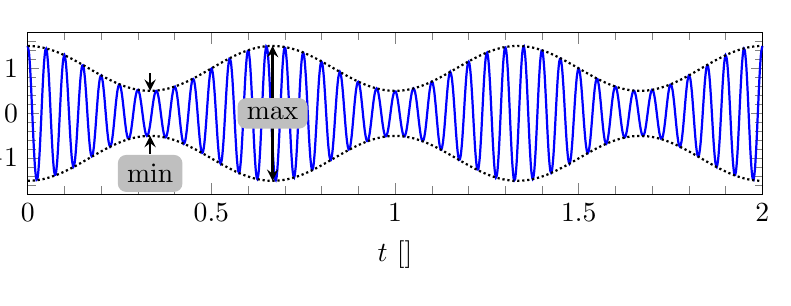
\begin{tikzpicture}[trim axis left, trim axis right]
  	\begin{axis}[
    	clip=false,
    	width=0.9\textwidth, height=0.3\textwidth,
    	xlabel={$t$ [\si{\second}]},
    	ylabel={Amplitude [\si{\volt}]},
    	xmin=0, xmax=\maxt,
    	xtick distance=0.5,
    	minor x tick num=4,
    	ytick distance=1,
    	minor y tick num=4,
    	legend style={cells={anchor=west}, legend pos=outer north east,},
    	]
      \addplot [domain=0:{\maxt}, samples=500, smooth, mark=none, thick, color=blue, solid] {cos(deg(2*pi*\fTraeger*x))*(1 + (\Modulationstiefe/100)*(cos(deg(2*pi*(\fSignal)*x))))};
      \addplot [domain=0:{\maxt}, samples=100, smooth, mark=none, thick, color=black, densely dotted, forget plot] {+1*(\Modulationstiefe/100)*cos(deg(2*pi*\fSignal*x)) + 1};
      \addplot [domain=0:{\maxt}, samples=100, smooth, mark=none, thick, color=black, densely dotted, forget plot] {-1*(\Modulationstiefe/100)*cos(deg(2*pi*\fSignal*x)) - 1};
    	\draw [thick, black, stealth-] ({0.5/\fSignal},{+1-(\Modulationstiefe/100)}) -- ({0.5/\fSignal},{+1-(\Modulationstiefe/100) + 0.4});
    	\draw [thick, black, stealth-] ({0.5/\fSignal},{-1+(\Modulationstiefe/100)}) -- ({0.5/\fSignal},{-1+(\Modulationstiefe/100) - 0.4}) node[below,fill=gray!50!white,rectangle,rounded corners=3pt]{min};
    	\draw [thick, black, stealth-] ({1/\fSignal},{+1+(\Modulationstiefe/100)}) -- ({1/\fSignal},{0});
    	\draw [thick, black, stealth-] ({1/\fSignal},{-1-(\Modulationstiefe/100)}) -- ({1/\fSignal},{0});
    	\path ({1/\fSignal},{+1+(\Modulationstiefe/100)}) -- node[fill=gray!50!white,rectangle,rounded corners=3pt]{max} ({1/\fSignal},{-1-(\Modulationstiefe/100)});
  	\end{axis}
	\end{tikzpicture}
\end{center}
